\documentclass[10 pt]{article}
\usepackage{tikz}
\usetikzlibrary{arrows}
\usepackage[margin=0.5 in]{geometry}
\usepackage[utf8]{inputenc}
\usepackage{tabu}
\usepackage{color}
\usepackage{xcolor}
\usepackage{listings}
\usepackage{enumitem}
\usepackage{multicol}
\usepackage{enumitem}
\usepackage{algorithm}
\usepackage{algpseudocode}
\usepackage{comment}
\setlength{\columnsep}{1cm} 
\title{\textbf {Estructuras de Datos 2 - ST0247\\Primer Parcial}}
\author{Nombre ..............................\\
		Departamento de Informática y Sistemas\\
		Universidad EAFIT\\}
\date{Marzo 22 de 2018}
\begin{document}
\lstdefinestyle{customc}{
	language=Java, 
	numbers=left, 
	showspaces=false,
    showstringspaces=false, 
    tabsize=2, 
    breaklines=true,
    xleftmargin=5.0ex,
}

\lstset{escapechar=@,style=customc, numbers=left, stepnumber = 1} 
\maketitle
\begin{multicols}{2}
\section{Permutaciones 30\%}
Calcular las permutaciones de un conjunto de enteros es un problema que surge continuamente en la Ingeniería de Sistemas. Calcular tales permutaciones es importante porque muchos problemas se resuelven simplemente probando cada una de las permutaciones para cierto conjunto de datos. Es por esto que a usted se le ha encomendado la tarea de encontrar todas las posibles permutaciones (no necesariamente en orden \textbf{\textit{Lexicográfico}}) que se pueden generar dado un conjunto de enteros. Al siguiente algoritmo le falta completar algunas líneas, por favor completa cada una de ellas. Un \textbf{ejemplo} de salida para e = \{1, 2, 3\} sería:
\begin{itemize}
\item 1, 2, 3
\item 1, 3, 2
\item 2, 1, 3
\item 2, 3, 1
\item 3, 1, 2
\item 3, 2, 1
\end{itemize}

Tengan en cuenta que el método \texttt{add(e)} agrega un elemento $e$ al final de una lista y el método \texttt{removeLast()}
elimina el último elemento de una lista.

\begin{lstlisting}
private void permutar(int[] e, 
    boolean[] incluido, 
    LinkedList<Integer> lista){  
  if(lista.size() == e.length){
    imprimirPerm(lista);
    return;
  }
  for(int i = 0; i < e.length; ++i){
    if(incluido[i] == ........){
      continue;    
    }  
    incluido[i] = true;
    lista.add(e[i]);
    permutar(e);
    incluido[i] = ..............;
    lista.removeLast();
  }
}

public void permutar(int[] e) {
  permutar(e, 
           new boolean[e.length], 
           new LinkedList<Integer>());	
}
\end{lstlisting}
\begin{enumerate}[label=(\alph*)]
\item (10\%) Complete la línea 13 .................
\item (10\%) Complete la línea 19 .................
\item (10\%) Asumiendo que $imprimirPerm(lista)$ se ejecuta en $O(1)$. ¿Cuál es la complejidad asintótica, en el peor de  los casos, del algoritmo anterior?
\begin{enumerate}[label=(\roman*)]
\item $O(n^2)$
\item $O(2^n \times n)$
\item $O(n!)$
\item $O(n^4)$
\end{enumerate}
\end{enumerate}
\section{DFS \& BFS 20\%}
Los ejercicios de esta sección se deberan resolver de acuerdo al siguiente grafo.
\\
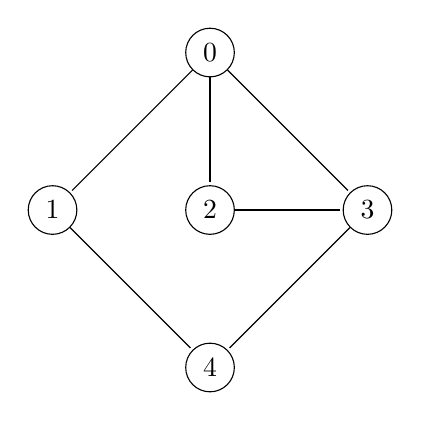
\begin{tikzpicture}[shorten >= 1 pt, auto]
\tikzset{vertex/.style = {shape=circle,draw,minimum size=1.5em}}
\tikzset{edge/.style = {> = latex'}}

\node[vertex] (B) at (2,4)  {0};
\node[vertex] (D) at (0, 2) {1};
\node[vertex] (E) at (2, 2) {2};
\node[vertex] (F) at (4, 2) {3};
\node[vertex] (G) at (2, 0) {4};

%edges
\draw[edge] (B) edge node{} (E);
\draw[edge] (B) edge node{} (D);
\draw[edge] (B) edge node{} (F);
\draw[edge] (D) edge node{} (G);
\draw[edge] (F) edge node{} (G);
\draw[edge] (E) edge node{} (F);

\end{tikzpicture}

\begin{enumerate}[label=(\alph*)]
\item (10\%) DFS. Un posible recorrido \textbf{\textit{DFS}} del grafo anterior, al ejecutarlo desde el vértice $0$, es:
\begin{enumerate}[label=(\roman*)]
\item $0, 4, 1, 2, 3$
\item $0, 2, 4, 3, 1$
\item $0, 1, 4, 3, 2$
\item $0, 4, 2, 3, 1$
\end{enumerate}
\item (10\%) BFS. Un posible recorrido \textbf{\textit{BFS}} del grafo anterior, al ejecutarlo desde el vértice $0$, es:
\begin{enumerate}[label=(\roman*)]
\item $0, 1, 2, 3, 4$
\item $0, 1, 4, 2, 3$
\item $0, 4, 3, 2, 1$
\item $0, 4, 2, 1, 3$
\end{enumerate}
\end{enumerate}
\section{Fuerza bruta 20\%}
Tenemos dos enteros, $M$ y $N$. Queremos contar en el rango $[M, N]$ todos los enteros que contienen los dígitos $a, b, c, d$ y $e$, $1 \leq a, b, c, d, e \leq 9$. Al siguiente algoritmo le faltan algunas líneas. Ayudanos a completarlas.
\begin{itemize}
\item \textbf{Ejemplo: } Considere $a = 1, b = 1, c = 4, d = 1, e = 4$ y el rango $[200, 300]$. Los enteros que cumplen la condición son: $214, 241$. Por lo tanto la solución debería ser $2$. 
\item \textbf{Nota: } Observe que $a, b, c, d, e$ no tienen que ser necesariamente distintos; además sólo importa que $a, b, c, d, e$ estén todos en el numero, es decir, si $S = \{d_1,d_2,d_3, ..., d_k\}$ es el conjunto de todos los dígitos de algún numero $N \leq x \leq M$ y $T = \{a, b, c, d, e\}$, siempre se cumple que $S \cap T = T$.
\end{itemize}
\begin{lstlisting}
public int contar(int N, int M){
	int total = 0;
	int[] set;
	for(int i = N; i <= M; ++i){
		set = new int[10];		
		int temp = i;
		while(temp > 0){
			int rem = ___________;
			set[rem] = set[rem] + 1;
			temp = temp / 10;		
		} 
		if(set[a] > 0 && set[b] > 0 && 
			set[c] > 0 && set[d] > 0 && 
			set[e] > 0){
			total = total + 1;		
		}
	}
	return total;
}
\end{lstlisting} 
\begin{enumerate}[label=(\alph*)]
\item (10\%) Complete la línea 8 ..............
\item (10\%) ¿Cuál es la complejidad del algoritmo?.
\begin{enumerate}[label=(\roman*)]
\item $O(|N - M|)$
\item $O(|N - M| \times \log_{10} M)$
\item $O(|N - M| \times N)$
\item $O(|N - M| \times M)$
\end{enumerate}
\end{enumerate}


\section{Voraces 30\%}
Considere el siguiente problema. El doctor le ha recomendado comer $a$ vitaminas, $b$ proteínas y $c$ minerales. Usted puede ir a un lugar donde hay infinitas cantidades de éstas tres cosas; además, usted no tiene que pagar por nada. Sin embargo, uno puede ir sólo una vez por día y cada día que uno va al lugar tiene que tomar una de estas dos posibilidades:
\begin{enumerate}
\item Tomar $3$ cosas distintas (vitaminas, proteínas y minerales), es decir puede tomar una vitamina, una proteína y un mineral;
\item Tomar $2$ cosas del mismo tipo, es decir, $2$ vitaminas, $2$ proteínas o $2$ minerales.
\end{enumerate}

Como usted está muy enfermo quiere saber cuál es la mínima cantidad de días que tiene gastar para ir a ese lugar para tener al menos $a$ vitaminas, $b$ proteínas y $c$ minerales. 

\textbf{Ejemplo: } Suponga que $a = 3, b = 4, c = 7$. La solución óptima sería ir los tres primeros días por $3$ cosas distintas. Luego los siguientes días ir por $2$ cosas iguales. Si se hace el cálculo se demostrará fácilmente que usted tiene que ir $3$ días seguidos por dos cosas distintas. Por lo tanto la solución sería $6$ días. Es decir, un posible recorrido con el mínimo número de viajes es el siguiente:

\begin{enumerate}
\item Ir por 1 vitamina, 1 proteína y 1 mineral
\item Ir por 1 vitamina, 1 proteína y 1 mineral
\item Ir por 1 vitamina, 1 proteína y 1 mineral
\item Ir por 2 proteínas
\item Ir por 2 minerales
\item Ir por 2 minerales
\end{enumerate}
{\footnotesize
\begin{lstlisting}
 int numeroDias(int a, int b, int c){
  //Intentar primero tomando de a 3
  int minimo = Math.min(a, Math.min(b, c));
  //Hay que quitarlas a cada variable
  a = a - minimo;
  b = b - minimo;
  c = c - minimo;
  //Ahora tomemos de a 2 cosas.
  int temp = a + b + c + 1;
  temp = __________________;
  return __________________;
 }
\end{lstlisting}
}
\begin{itemize}
\item \textbf{Pista 1: } La forma óptima de ir por tres cosas cada día es solo cuando tengo que ir por de las tres cosas, es decir, cuando $a > 0 \land b > 0 \land c > 0$. La mejor forma de ir por dos cosas cada día es cuando solo tengo que ir por a lo sumo dos cosas, es decir, $a = 0 \lor b = 0 \lor c = 0$.
\item \textbf{Pista 2: } Verifique que $a = minimo \lor b = minimo \lor c = minimo$.
\end{itemize}
Por favor complete las siguientes líneas:
\begin{enumerate}[label=(\alph*)]
\item (10\%) Complete la línea 10 .................
\item (10\%) Complete la línea 11 .................
\item (10\%) ¿Cuál es la complejidad del método anterior?
\begin{enumerate}[label=(\roman*)]
\item $O(n)$
\item $O(1)$
\item $O(n^2)$
\item $O(n \log n)$
\end{enumerate}
\end{enumerate}



\end{multicols}

%Respuestas 1:
%(a) true
%(b) false
%(c) (iii) O(n!)
%Respuestas 2:
%(a) (iii) 0, 1, 4, 3, 2
%(b) (i)   0, 1, 2, 3, 4
%Respuestas 3:
%(a) temp % 10
%(b) (ii) O(|N-M|) x log(10) m

% 4. Voraces
% (a) temp / 2
% (b) temp + minimo
% (c) (ii)
\end{document}